\documentclass{cmc}
\usepackage{makecell}
\usepackage{enumitem}
\usepackage{amsmath}
\usepackage{float}
\usepackage{amsmath}
\usepackage{algorithm}
\usepackage{hyperref}
\usepackage[noend]{algpseudocode}
\usepackage{forest}
\usepackage{url}

\hypersetup{
    colorlinks=true,
    linkcolor=blue,
    urlcolor=blue,
    citecolor=blue
}

\makeatletter
\def\BState{\State\hskip-\ALG@thistlm}
\makeatother
\begin{document}

\pagestyle{fancy}
\lhead{\textit{\textbf{Computational Motor Control, Spring 2026} \\
    Project 1, GRADED}}

\begin{center}
{\huge\bfseries Amphibious Locomotion of Polymander} \\[0.5em]
{\LARGE A Salamander-like Robot}
\end{center}

\tableofcontents
%share

\section{Introduction}\label{sec:exploring-swimming}

In earlier practicals, we learned the basics of numerical integration, simulated a pendulum with passive properties, and modeled oscillator dynamics of a 2-neuron network. This project aims to combine and extend those concepts to implement a more comprehensive controller based on Central Pattern Generators (CPGs) and deploy it on a salamander-like robot - Polymander - to achieve aquatic and terrestrial locomotion.

A realistic neuromechanical model integrates neural control with
the biomechanical properties of robot body and its interaction with the fluid environment. Such a model allows us to systematically test how different neural parameters affect locomotion performance.

In \textbf{Project 1}, you will focus on modeling and simulating the swimming behavior of the robot. You will start with a simple wave controller and implement the evaluation metrics. You will then design a CPG controller to propel the robot to swim. In the end, you will add sensory feedback to the CPG network and study its role in the robot locomotion.

In \textbf{Project 2}, you will extend this controller to the walking gait.

\subsection{Embodiment}
Polymander \cite{fu2026polymander2} is a reconfigurable amphibious fish-like robot that could mimic both the \textit{Polypterus} (a fish that can walk on land and has a bipedal body plan) and \textit{Salamander} (quadruped body plan). In this project, we are using its quadruped body plan and focusing on its representation of \textit{Salamander}. Polymander consists of 11 modular axial body segments, including a head, a front girdle and a hind girdle, six axial modules, and a tail module of two parts. For each girdle, it supports two attachable limbs made  of a leg module and a foot module ending in a silicone ball-shaped foot.

\begin{figure}[H]%
  \centering
    {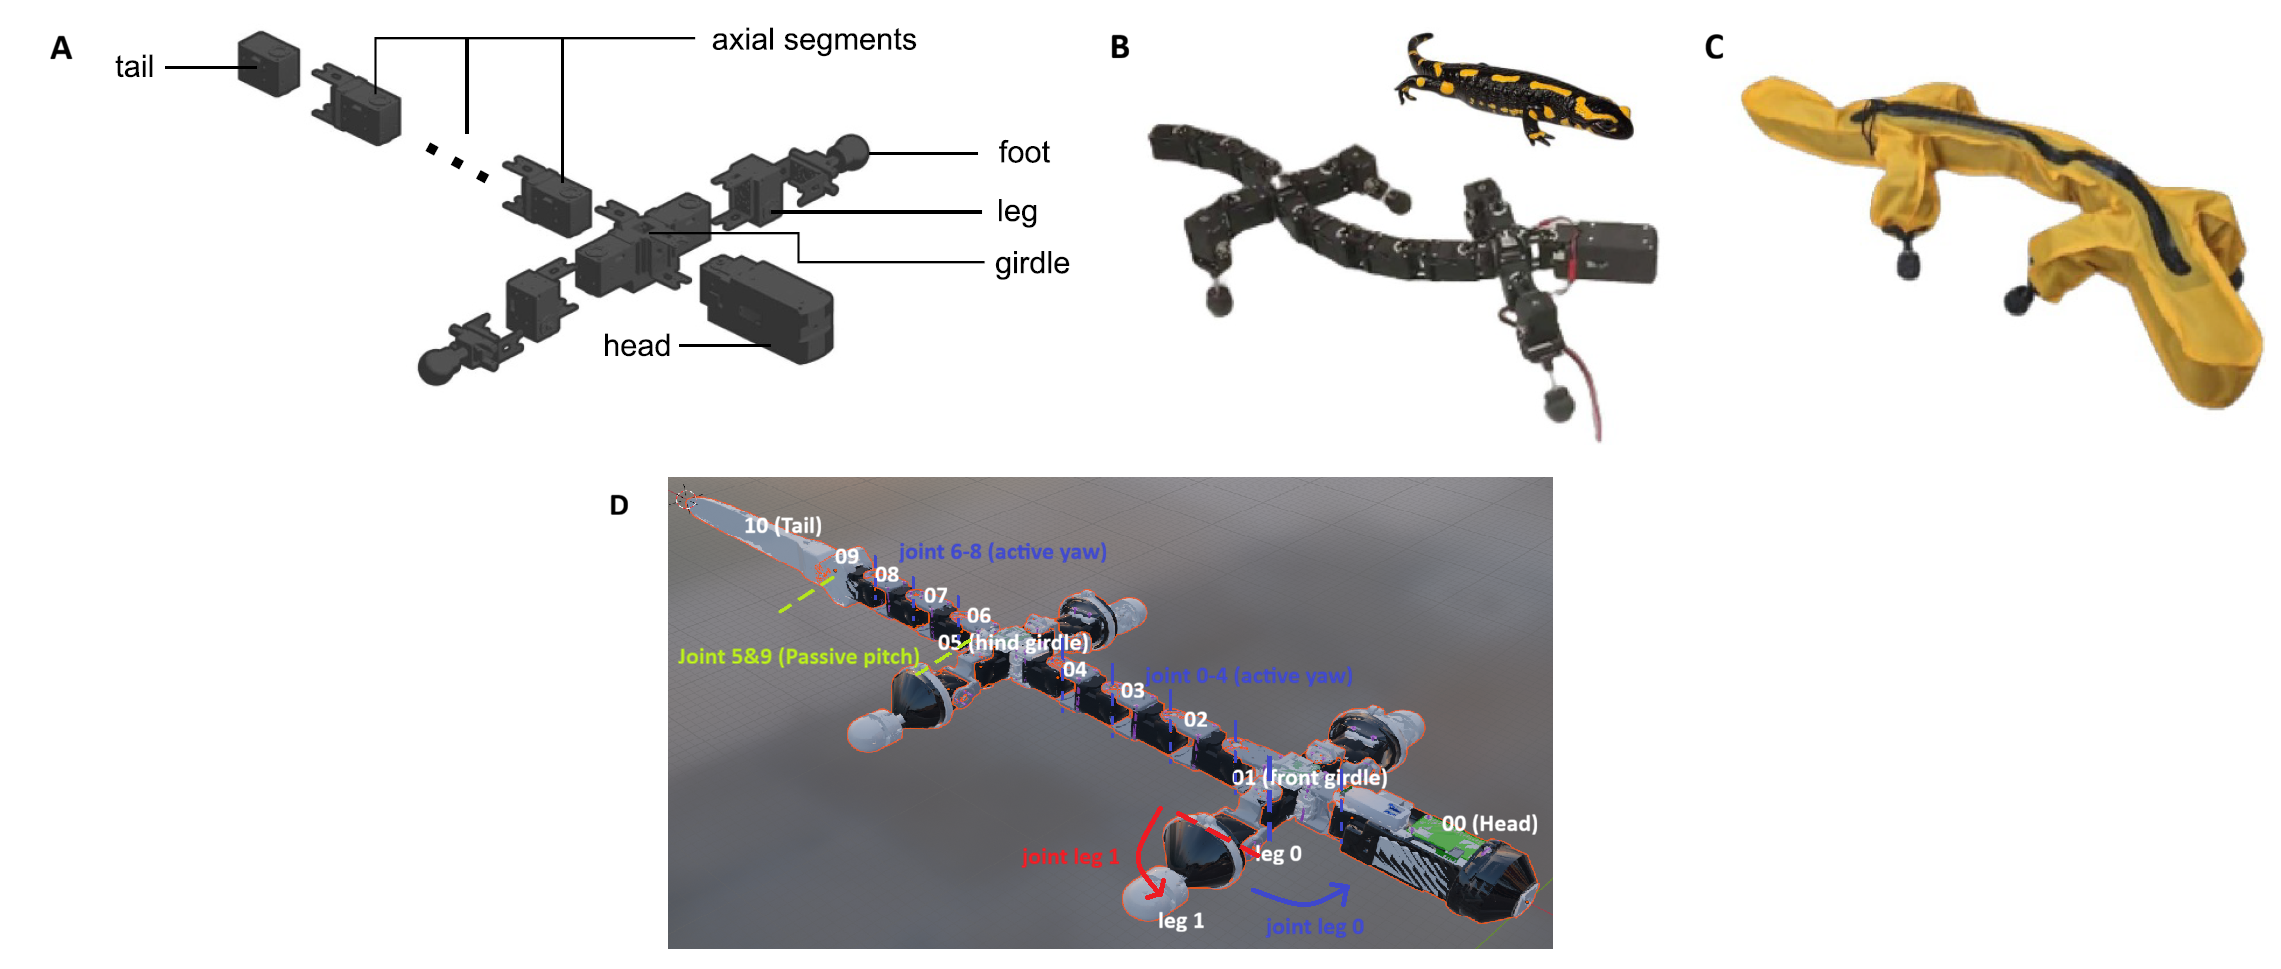
\includegraphics[width=\textwidth]{figures/Polymander robot.png}}
    \caption{Polymander Robot. (A) Reconfigurable modules of the robot. (B) Salamander configuration with two forelimbs and two hindlimbs. (C) Polymander inside its waterproof suit. (D) Links and joints definition of Polymander in the quadruped plan.}
\end{figure}

Along the body axis, the Polymander model consists of $n_{links}=11$ links connected by $n_{joints}=10$ rotational joints. The joints are numbered from 0 to 9, ordered from the head to the tail. Besides joint 5 and joint 9 that are passive pitch joints moving up and down, all other joints are actively controlled yaw joints that move left and right. For each limb, it has one active joint connecting the girdle and the leg module that moves forward/backward (abduction/adduction) and one active joint connecting the leg module and the foot module that swings downward/upward (flexion/extension).

To imitate the swimming behavior of real animals, the torque produced by the servo motors at each actively controlled joint is computed by means of Ekeberg muscle models (that will be explained in a lecture). For each joint, the model receives in input the left ($M_{L_i}$) and right ($M_{R_i}$) activations from the muscle cells, the current joint angle ($\theta_i$) and joint speed ($\Dot{\theta_i}$) to compute the resulting output torque ($\tau_i$) via:

  \[
	\tau_i = \alpha_i M_{diff_i} + \beta_i(\gamma_i +M_{sum_i} )\theta_i + \delta_i \Dot{\theta_i} \\
  \]
  \[
    M_{diff_i} = (M_{L_i} - M_{R_i}) \\
  \]
  \[
    M_{sum_i} = (M_{L_i} + M_{R_i})
  \]

Where $\alpha_i$ is the active gain, $\gamma_i$ is the passive stiffness, $\beta_i$ is the active stiffness, $\delta_i$ is the damping coefficient. The Ekeberg muscle model is a rotational spring-damper system with the addition of a variable stiffness term $\beta (M_L+M_R) \theta_i$. The neutral position of the stiffness is fixed at zero for spine joints and at an extended position for limb joints for Project 1. The active term of the model acts an external torque $\alpha(M_L-M_R)$. You do not need to optimize the muscle parameters, and \texttt{muscle\_params.csv} contains the tuned muscle parameters ready for use. We assume robot motors in the simulation to be ideal and do not account for real motor non-linearities and dynamics.

When submerged in water, the body is subjected to buoyancy and hydrodynamic forces. Buoyancy forces are applied to each link according to its submerged volume $V_{UW}$

  \[
	\mathrm{F_{b_i}} = V_{UW_i} \rho g
  \]

Where $\rho$ is the water density and $g$ is the gravity acceleration ($g = 9.81 m/s^2$).
We consider the swimming of the robot in high Reynolds number regimes and opted for a simplified hydrodynamic model composed of inertial drag forces. For each link, a speed-dependent drag force ($F_d$) is applied in each dimension ($i$) according to:

  \[
	\mathrm{F_{d_i}} = \frac{1}{2} \rho C_{d_i} A_{i} V_{i}^2
  \]

Where $A$ is the link's cross-sectional area, $c_{d_i}$ is the drag coefficient in the i-th dimension, $V_{i}$ is the current speed of the link in the i-th dimension in the reference frame of the center of mass of the link. The drag coefficients were chosen to match the swimming speed of Polymander in real life in its swimming suit when replaying the swimming kinematics. You do not need to tune the drag coefficients, and they are pre-defined in the model.


\subsection{Code Structure}
The code is hosted at \texttt{https://gitlab.com/farmsim/courses/cmc-2026-students}. The \texttt{README.md} gives details on the installation. The files you need to change are marked in \textcolor{red}{red} and the lines to complete are tagged with \textcolor{red}{\texttt{\#TODO}} in each part of the assignment. Generated outputs (controller states, evaluation metrics, figures, videos) for each assignment should be saved to \texttt{logs/exercise\_\{assignment number\}} folder.

Optionally, you could create plotting utilities in \texttt{cmc\_controllers/plot\_utils.py} and use them in the main assignment files. Unless necessary and well motivated, no additional dependencies shall be added to the environment.
%matplotlib and seaborn

\subsection{Report Structure}

Include a short report including plots and results addressing the questions stated under each assignments (see below). You do not need to repeat the methodology that already exists in this file, rather your own methods and results that you generated. The report has to be no longer than 8 pages, excluding references, generative AI declaration and supplementary material. For supplementary material, we allow 2 additional pages in case you have extra diagrams to show but the main plots and graphs should be in the main report.
% This project is XXX of the total grade and the report needs to be submitted by XXX 23:59.


\subsection{Submission}
\textbf{Deadline:} The Project 1 needs to be handed in by \corr{\textbf{\underline{Wednesday, 29.04.2026 at 23:59.}}}

When submitting, zip your report and your code together as
\nolinkurl{cmc_project1_group_{group_number}.zip}, using your group
number in the filename. Your code should include code files only. The
virtual environment (e.g.\ the \texttt{venv} directory), the
\texttt{farms} folder, and the \texttt{logs} folder should
\textcolor{red}{not} be included. Videos and presented results in the
report should be reproducible by running the main exercise scripts.
Videos should have assignment numbers as prefixes and descriptive
phrases as suffixes that you refer to in your report. The structure of
your submission folder should look like below. The files marked with
\texttt{*} are the files to modify in the project.

\newpage

\begin{lstlisting}[basicstyle=\ttfamily\small]
cmc_mp1_group_{group_number}_name1_name2_name3.zip*
|-- cmc_mp1_group_{group_number}_name1_name2_name3.pdf*
\-- cmc_controllers/
    |-- neural_data.py
    |-- neural_options.py
    |-- polymander_controller.py
    |-- metrics.py*
    |-- wave_controller.py*
    \-- CPG_controller.py*
|-- exercise1_1.py*
|-- exercise1_2.py*
|-- exercise2_1.py*
|-- exercise2_2.py*
|-- exercise2_3.py*
|-- exercise3_1.py*
|-- exercise3_2.py*
|-- exercise3_3.py*
\-- videos*
    \-- ...

\end{lstlisting}

\noindent
\subsection*{Pro tips}\label{subsec:tips}

\begin{itemize}
\item \corr{\textbf{Check the notes on the code}}. Many explanations are given therein.
\item \corr{Be concise and precise} in the answers to the exercises. Do not repeat the methodology existing in this file.
\item  Back up your conclusion with \corr{videos} and \corr{Figures} to make your reasoning compact and strong.
\end{itemize}

\newpage

%%%%%%%%%%%%%%%%%%%%%%%%%%%%%%%%%%%%%%%%%%%%%%%%%%%%%%%%%%%%%%%%%%%%%%%%%%
% QUESTIONS %%%%%%%%%%%%%%%%%%%%%%%%%%%%%%%%%%%%%%%%%%%%%%%%%%%%%%%%%%%%%%
%%%%%%%%%%%%%%%%%%%%%%%%%%%%%%%%%%%%%%%%%%%%%%%%%%%%%%%%%%%%%%%%%%%%%%%%%%

\newpage
\section {Assignment}

\subsection{Wave Controller and Metrics} \label{subsec:wavecontroller}
Before implementing the CPG controller with couplings, we start by implementing a basic wave (i.e. sine) controller that generates a periodic traveling wave along the axial joints of the robot. The wave controller is designed with the intuition that the robot joints exhibit a traveling wave during swimming behaviors. When the active torque of the muscle dominates, the wave-like torque would likely induce acceleration, velocity, and joint pose close to a wave-like pattern that would propel the robot forward.

The wave controller is implemented such that:
\begin{itemize}
    \item All axial joints maintain the same cocontraction level of 2.0 during swimming as in Eq.\ref{eq:wave_controler_cocontraction}
    \item Active torques generated by axial joints form a periodic traveling wave as in Eq.\ref{eq:wave_controler_diff}.
\end{itemize}


\begin{align}
\label{eq:wave_controler_cocontraction}
    M_{sum_i} (t) &= M_{L_i} (t) + M_{R_i} (t) \nonumber\\
    &= 2
\end{align}

\begin{align}
\label{eq:wave_controler_diff}
M_{\mathrm{diff}_i}(t)
  &= M_{L_i}(t) - M_{R_i}(t) \nonumber \\
  &= A \cdot \sin\!\left(
      2\pi \left(
        f t - \epsilon\,\frac{i}{N_{\mathrm{joints}}}
      \right)
    \right)
\end{align}

where $\epsilon$ is the total wave lag, $A$ is the amplitude and $f$ is the frequency of the wave.

\textbf{\underline{Question 1.1} Complete your implementation of \fileref{WaveController()} in \fileref{cmc\_controllers/\\wave\_controller.py} marked with \textcolor{red}{TODO}. Run \fileref{scripts/exercise\_1.1.py} to initiate an instance of your wave controller with $A=2$, $f=2Hz$, $TWL=1$ to use it to simulate the robot swimming. Set \texttt{recording} to True and record a video of the swimming behavior.}

To analyze and study the locomotion behavior of the robot under different controller parameters. We define two kinds of metrics to quantify the simulation result in \fileref{cmc\_controllers/metrics.py}. The \textbf{Neural Metrics} (\textbf{NM}) quantifies the neural signals generated by the controller (we consider the difference between left and right muscle activation to be the neural signal per joint). The \textbf{Mechanical Metrics} (\textbf{MM}) quantifies how effectively and efficiently the body segments/joints move.

We define the following metrics in \texttt{metrics.py}.

\begin{itemize}
  \item \textbf{\underline{NM1}: }\textit{Neural frequency} (\(f_{\mathrm{neur}}\)) and \textit{Neural amplitude} (\(A_{\mathrm{neur}}\)):

  The frequency and the amplitude of a neural signal are computed via a Fast Fourier Transform (FFT).
  \[
    f_{\mathrm{neur}} = < \underset{f}{\mathrm{argmax}}\;\bigl|X_i[f]\bigr| >_i
  \]
  \[
    A_{\mathrm{neur}} = <\frac{2\,\bigl|X_i[k^i_{\text{max}}]\bigr|}{N} >_i
  \]
  where \(\bigl|X_i[k^i_{\text{max}}]\bigr|\) is the magnitude of the FFT at the index corresponding to the dominant frequency for each signal, and \(N\) is the number of samples.

  \item \textbf{\underline{NM2}: }\textit{Intersegmental phase lag ($IPL_{neur}$):}

  Intersegmental phase lag is used to quantify the phase difference among oscillating signals from different body segments. For two sinusoidal signals oscillating at similar frequencies, the delay \(\Delta t_{1,2}\) is computed by cross-correlation:
  \[
    \Delta t_{1,2}\;=\;\underset{\tau}{\mathrm{argmax}}\;\bigl(\mathrm{corr}\bigl(x_1,\,x_2\bigr)\bigr)
  \]

  The corresponding phase lag is computed by normalizing the delay by the average frequency of the two signals \(f_{1,2}\), as:
  \[
    PL_{1,2} \;=\; 2\pi\,f_{1,2}\;\Delta t_{1,2},
  \]

  Finally, the overall intersegmental phase lag is computed by averaging the phase lag values for each successive couple of signals along the body:

    \[
    IPL_{neur} \;=\; \frac{1}{N-1} \sum_{i=0}^{n-2} PL_{i, i+1}
    \]
\textbf{Note:} The phase lag of non-neural signals (e.g. mechanical joint angles) can be computed similarly.


    \item \textbf{\underline{MM1}: } \textit{Mechanical frequency ($f_{mech}$) and amplitude ($A_{mech}$).}

    These metrics are computed analogously to their neural counterparts, considering the joint angles instead of the muscle commands.

    \item \textbf{\underline{MM2}: }\textit{Forward speed ($v_{fwd}$,$v_{fwd(t)}$) and lateral speed ($v_{lat}$,$v_{lat(t)}$).}

    At each time step, we project the center-of-mass velocity \(\mathbf{v}_{\mathrm{COM}}(t)\) onto the forward ($d_{fwd}(t)$) and lateral ($d_{lat}(t)$) principal axes of the robot.
    The overall speed metrics are computed by averaging the instantaneous values over time:

    \[
    v_{\mathrm{fwd}} \;=\; <\mathbf{v}_{\mathrm{COM}}(t)\,\cdot\,\mathbf{d} _{\mathrm{fwd}(t)} >_t
    \]
    \[
    v_{\mathrm{lat}} \;=\; <\mathbf{v}_{\mathrm{COM}}(t)\,\cdot\,\mathbf{d}_{\mathrm{lat}(t)} >_t
    \]
    \begin{figure}[H]%
    \nonumber
      \centering
        {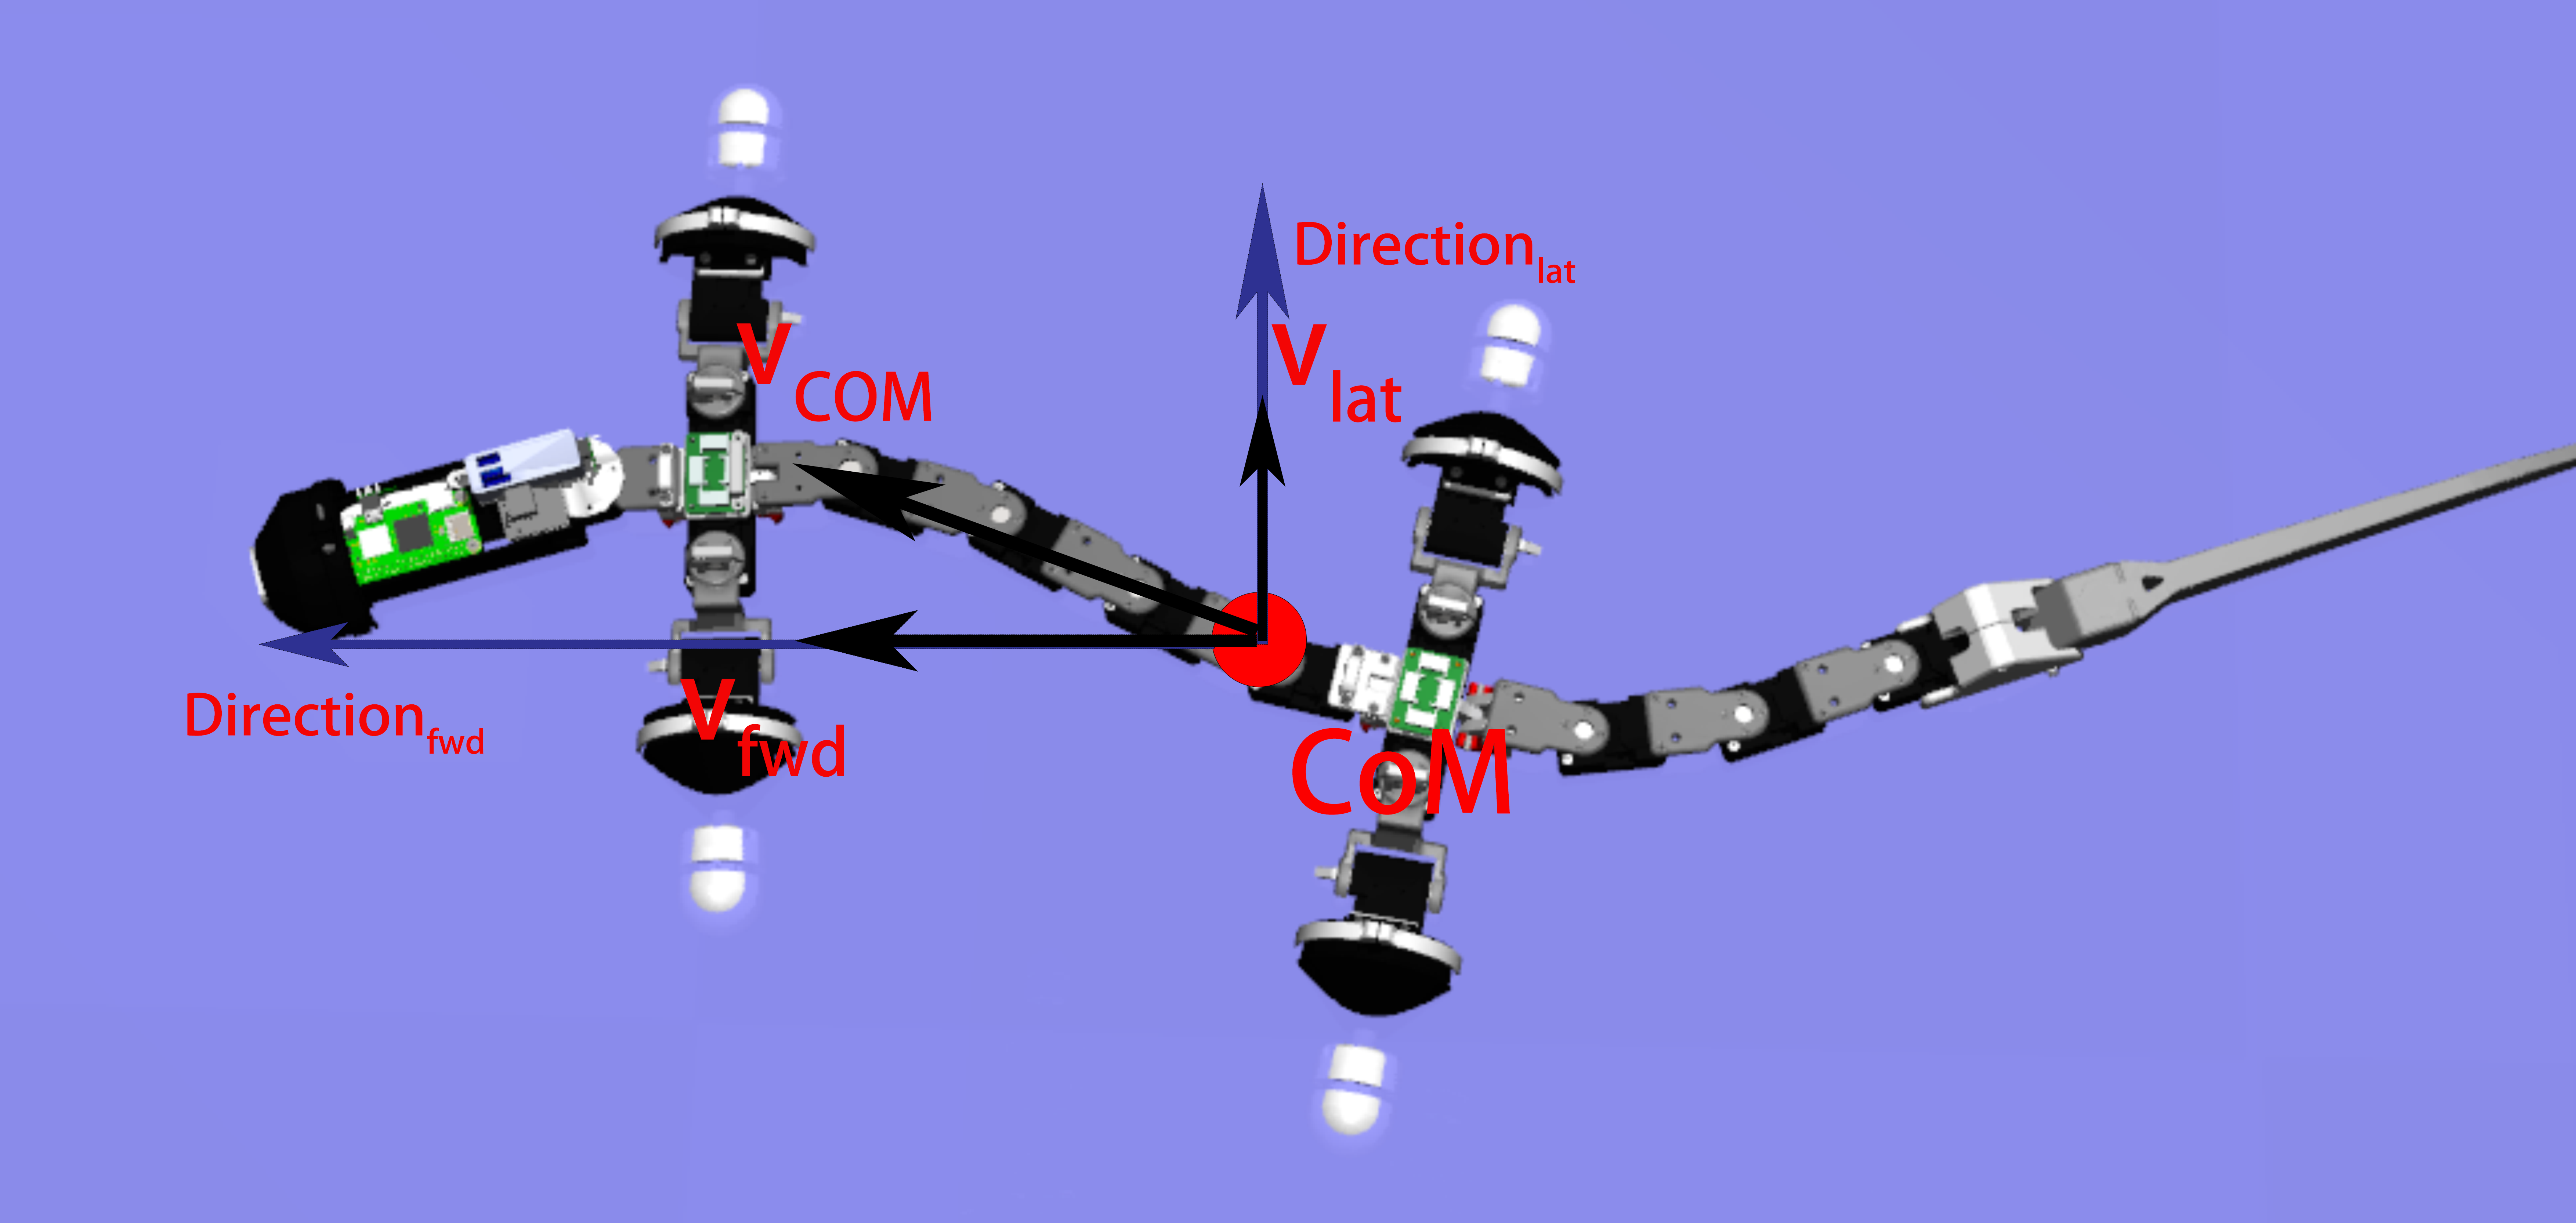
\includegraphics[width=.6\textwidth]{figures/metrics_velocity.png}}
    \end{figure}

    \item \textbf{\underline{MM3}: }\textit{Curvature \(\kappa\)}

    Curvature is used to evaluate the straightness of the robot trajectory. For a trajectory in 2D, the curvature is
    \[
    \kappa = \frac{\dot{x}\ddot{y}-\ddot{x}\dot{y}}{(\dot{x}^2+\dot{y}^2)^{3/2}}
    \]
    where $\dot{x}$ and $\dot{y} $ are the speed components.

    A large curvature indicates a sharp turning direction, while a small curvature indicates a straighter line. The sign indicates the turning direction.

    \item \textbf{\underline{MM4}: }\textit{Energy consumption (\(E\)) and Cost of transport (CoT).}

    We compute energy as an integration of the positive power \(\tau_j(t)\,\dot{\theta}_j(t)\) at each joint. We do \textbf{not} model energy recovery from negative work.

    \[
    P_j(t) \;=\;\max\bigl( \; \tau_j(t)\,\dot{\theta}_j(t),\, \;0 \bigr)
    \]
    \[
    E \;=\;  dt \times \sum_{t} \sum_{j=1}^{n} P_j(t)
    \]

    The cost of transport relates the energy expenditure to the distance traveled.
    \[
    \text{CoT} \;=\;\frac{E}{D_{\mathrm{fwd}}},
    \]
    where \(D_{\mathrm{fwd}}\) is the forward distance covered by the center of mass (CoM).

\end{itemize}

\textbf{\underline{Question 1.2} Complete the implementation of metrics \underline{NM2} ($IPL_{neur}$), \underline{MM2} ($v_{fwd}$ and $v_{lat}$), \underline{MM4} ($CoT$ and $E$) in \fileref{cmc\_controllers/metrics.py}. Modify \texttt{post\_processing()} in  \\ \fileref{cmc\_controllers/exercise\_1.1.py} to load the simulation result from your wave controller and evaluate its performance. Do they match your expectations? Plot the time evolution of joint angles for a few cycles and the CoM trajectory of the robot during swimming in 2D.
}


\textbf{\underline{Question 1.3} Explore the effect of different wave controller parameters on the performance metrics of the robot locomotion in \fileref{cmc\_controllers/exercise\_1.2.py}. Simulate the robot swimming and perform a 2D-grid parameter investigation of \underline{$A \in [1.0,4.0]$,} \\ \underline{$TWL \in [0.2,1.5]$   and $f =1.5 Hz$}. Qualitatively analyze the effect on the forward speed, CoT, average $IPL_{neur}$, and average $\phi_{lock}$.
}

\textbf{Hint:} For running several controllers with different hyperparameters in parallel, you could use \texttt{run\_multiple()}. Adjust max workers depending on your hardware capacity. This function would be useful in later exercises.



\subsection{CPG controller}

Here, we first describe the equations of the CPG network you will implement to control the Polymander robot (replacing the wave controller of the previous section). Each active joint (body and limb) is governed by a pair of oscillators representing the extensor and flexor in real muscle configuration. In total, we consider a double-chain oscillator with $n_{cpg\_body}=16$ oscillators along the body and $n_{cpg\_limb}=16$ oscillators distributed over 4 limb. During swimming, the limb network is considered to be saturated with zero amplitude and \textbf{we consider only the axial network in Project 1}. An illustration of the network is shown as in Fig \ref{fig:model_controller}.

\begin{figure}[H]
  \centering 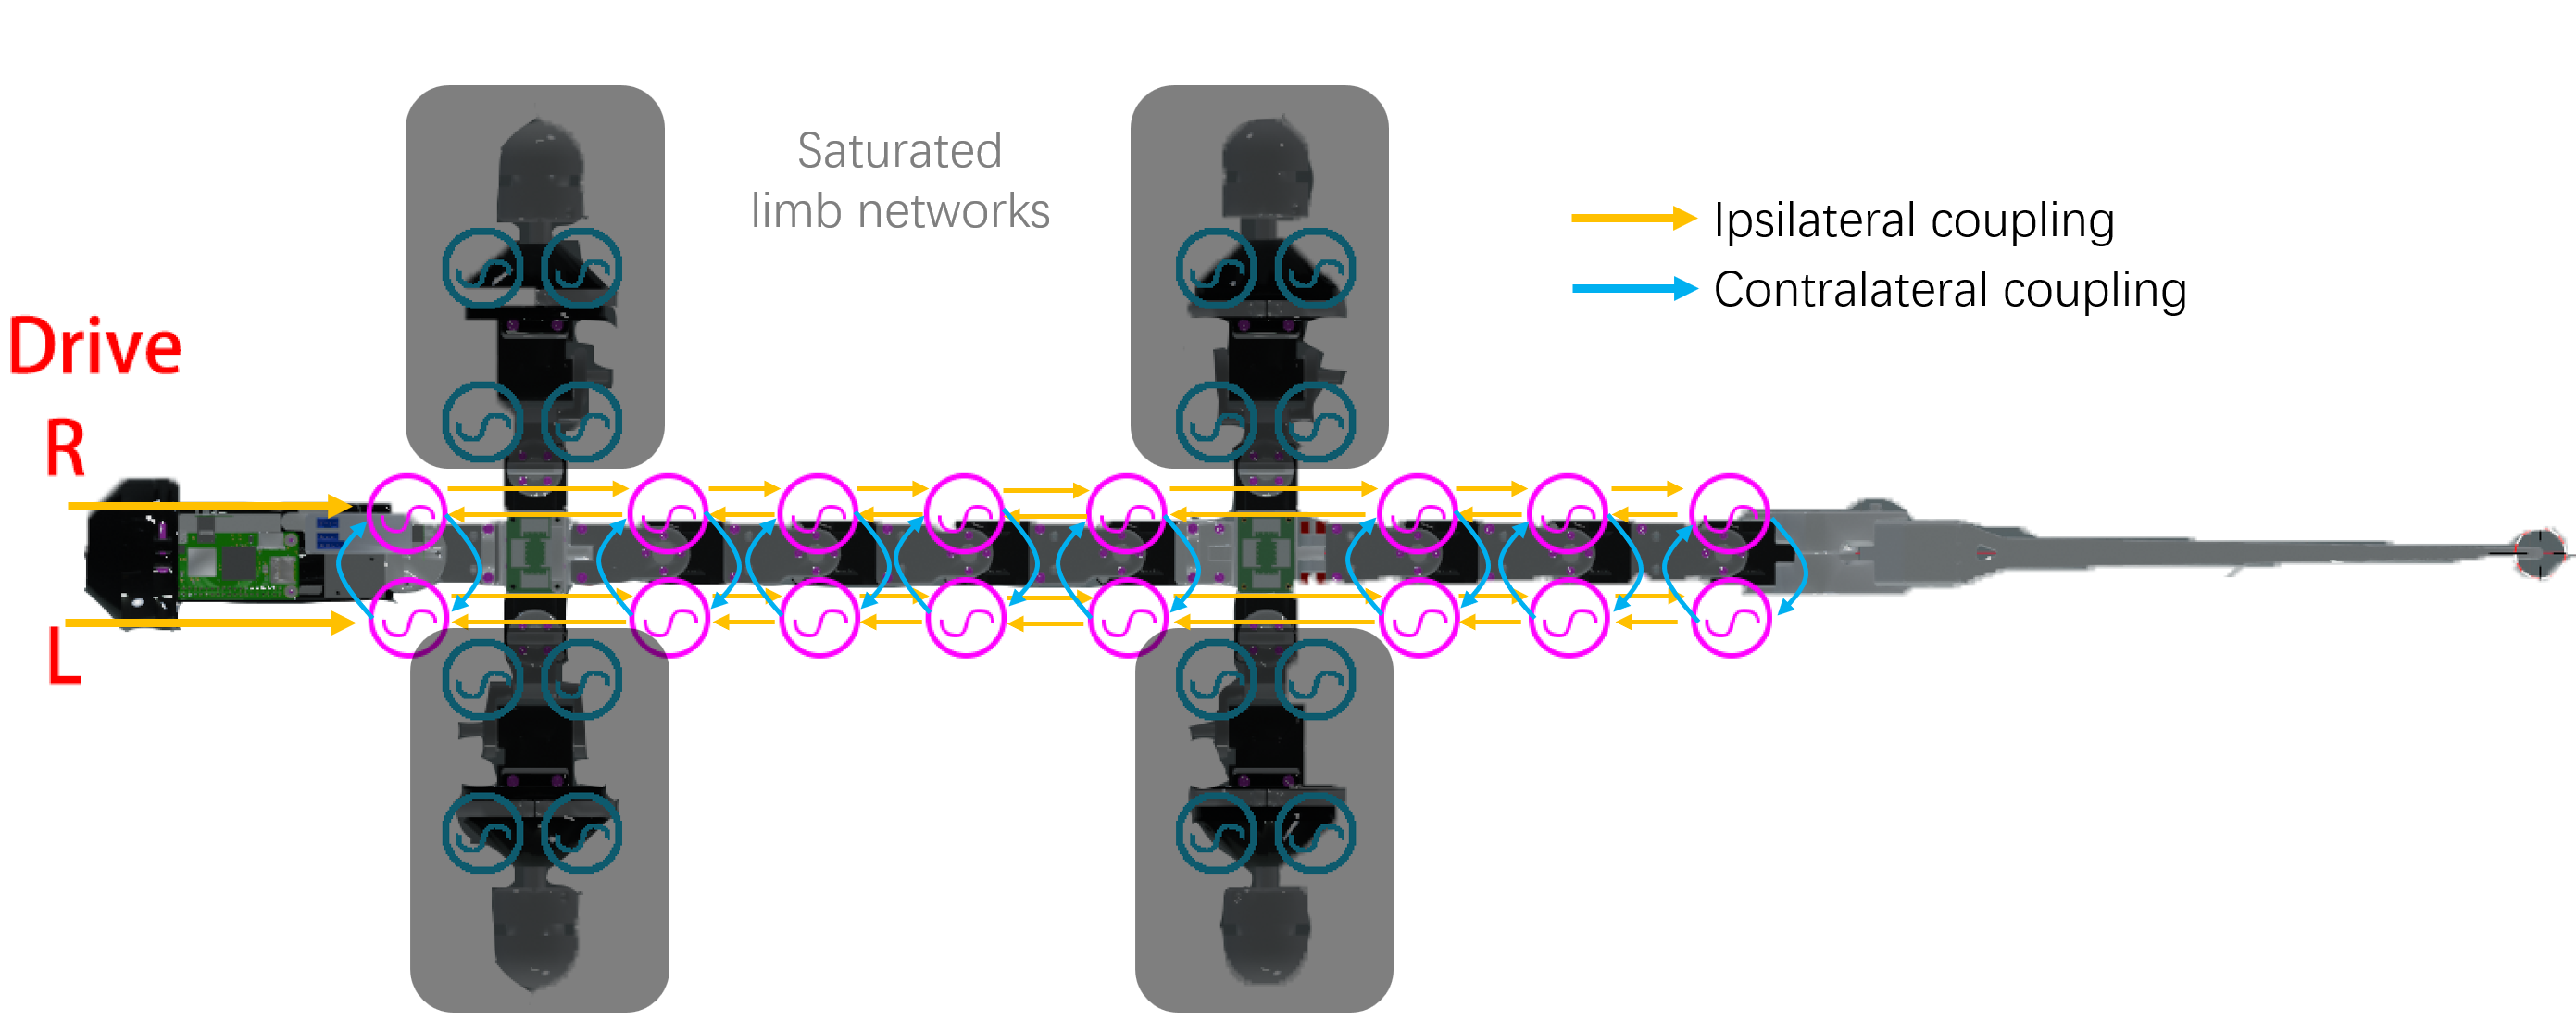
\includegraphics[width=.8\textwidth]{figures/network swimming.png}
  \caption{\label{fig:model_controller} Configuration of the spinal CPG controller in Polymander. Limb networks are saturated and not considered in Project 1. Axial active joints are driven by 8 pairs of Ekeberg muscles receiving motor outputs from a double chain of 16 oscillators with ipsilateral and contralateral coupling. The CPG model receives descending signals from the drive representing the brain MLR region in real animals.}
\end{figure}

The oscillator's phase equation is defined in Eq.\ref{eq:dphase}, with $ \theta_i $ the oscillator phase, $f_i$ the oscillator intrinsic frequency, $ w_{ij} $ the coupling
weights, $ \phi_{ij} $ the nominal phase lag (phase bias), $ r_i $ the
oscillator amplitude.
\begin{equation}
  \label{eq:dphase}
  \dot{\theta}_i = 2 \pi f_i + \sum_j r_j w_{ij} sin(\theta_j - \theta_i - \phi_{ij})
\end{equation}

In this model, we only consider couplings between ipsilateral (i.e. successive same-side oscillators) and contralateral (i.e. left-right) oscillators as in Eq.~\ref{eq:dcw}.

\begin{equation}
  \label{eq:dcw}
  w_{ij} =
    \begin{cases}
    w_{body2body\_rostral},& \text{if i,j are \color{orange}adjacent oscillators from tail to head} \\
    w_{body2body\_caudal},& \text{if i,j are \color{orange}adjacent oscillators from head to tail} \\
    w_{body2body\_contra}, & \text{if i,j are \color{blue}opposite oscillators on the other side}\\
    0, & \text{otherwise} \\
    \end{cases}
\end{equation}


The nominal phase lags are defined in Eq.~\ref{eq:phicw}, such that the phase lags between contralateral segments are constant $\pi$ and the phase lags between ipsilateral segments are constant values $PB_{i,j}$ that sum up to $\phi_{body\_total}$ from head to tail.


\begin{equation}
  \label{eq:phicw}
  \phi_{ij} =
    \begin{cases}
    PB_{i,j},& \text{if upwards (ipsilateral)} \\
    -PB_{i,j},& \text{if downwards (ipsilateral)}\\
    \pi,& \text{if left to right (contralateral)}\\
    -\pi,& \text{if right to left (contralateral)}\\
    0, & \text{otherwise} \\
    \end{cases}
\end{equation}
where
\[
    \sum_{i=0}^{n_{joint}-1} PB_{i,j}=\phi_{body\_total}\;
\]

The oscillator's amplitudes are defined in Eq.~\ref{eq:dr}, with $ r_i $ the
oscillator amplitude, $ R_i $ the nominal amplitude and $ a_i $ the convergence rate of nominal amplitudes. Note that this equation is actually the same equation as in \cite{ijspeert2007swimming} and has been simplified into a first-order ODE in order to simplify the implementation in this project.

\begin{equation}
  \label{eq:dr}
  \dot{r}_i = a_i (R_i - r_i)
\end{equation}

The oscillator frequency (Eq.~\ref{eq:freq}) and nominal amplitudes per joint (Eq.~\ref{eq:amp}) are defined in Eq.~\ref{eq:amp} as linear functions of drive $d$ with an offset and a lower/upper saturation bound as in \cite{ijspeert2007swimming} to simulate that the CPG controller can be receive descending commands from a higher level controller (brain commands in the real animal). Similarly to the real animal, an increasing descending drive tends to increase both the frequency and amplitude of muscle contractions (within some saturation limits $d_{low}$ and $d_{high}$) and therefore faster swimming.

\begin{equation}
  \label{eq:freq}
  f_i =
    \begin{cases}
        0 & \text{if $d<d_{low}$ or $d>d_{high}$} \\
        G_{freq_i}\cdot (d-d_{low})+c_{f_i,0},& \text{Otherwise}
    \end{cases}
\end{equation}

\begin{equation}
  \label{eq:amp}
    R_i =
    \begin{cases}
        0 & \text{if $d<d_{low}$ or $d>d_{high}$} \\
        G_{amp\_i}\cdot (d-d_{low})+c_{R_i,0},& \text{Otherwise}
    \end{cases}
\end{equation}

\begin{figure}[H]
  \centering 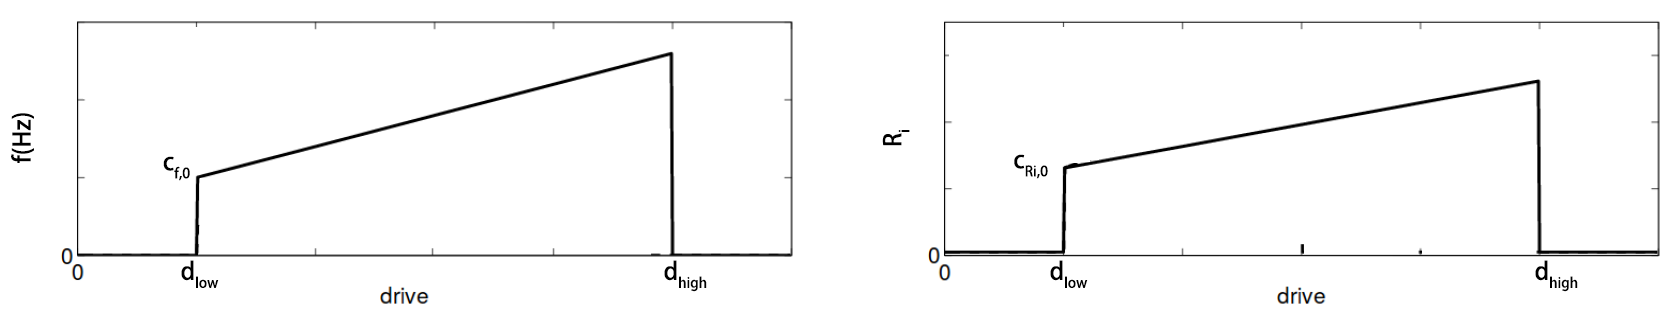
\includegraphics[width=.95\textwidth]{figures/drive.png}
  \caption{\label{fig:drive} Axial oscillator properties as a function of drive. Reference: \cite{ijspeert2007swimming}}
\end{figure}

The oscillator phases and amplitudes evolve with Euler numerical integration as in Eq.~\ref{eq:ode}.

\begin{equation}
\label{eq:ode}
\begin{aligned}
  r_{i_{t+1}} &= r_{i_t} + \dot{r}_{i_t}\cdot \Delta t \\
  \theta_{i_{t+1}} &= \theta_{i_t} + \dot{\theta}_{i_t}\cdot \Delta t
\end{aligned}
\end{equation}

Finally, the muscle output of an oscillator is defined as a function of oscillator phase and amplitude in Eq.~\ref{eq:output_body}.

\begin{equation}
  \label{eq:output_body}
  M_i = r_i(1 + cos(\theta_i))
\end{equation}

\textbf{\underline{Question 2.1} Complete \fileref{cmc\_controller/CPG\_controller.py} to implement the CPG controller with the default parameters in Tab.~\ref{tab:cpg_params}. Modify the \texttt{\_\_init\_\_} function to initialize the CPG nominal amplitudes, frequencies, coupling weights, and phase biases. Modify the \texttt{network\_ode} and \texttt{step} function to implement the ODE and derivative updates. Test your implementation by running the network using \fileref{cmc\_controllers/exercise2.1.py}. Record a video of the working controller with fixed drives of $d_{left}=d_{right}=3$ . Plot the time evolution of oscillator states ($\theta$ and $r$), sum and difference of muscle outputs ($M_{L_i}+M_{R_i}$),($M_{L_i}-M_{R_i}$), body joint angles, and robot CoM trajectory in 2D for the first 5s of the simulation.
}

\textbf{Hint:} For oscillator states that need frequent updates (e.g. amplitudes and their derivatives), initialize a \texttt{state} array and compute the ODE update of \texttt{state} array in \texttt{network\_ode} function. For oscillator parameters that are fixed once initiated (e.g. coupling weights), compute them once in \texttt{init} and retrieve later in \texttt{network\_ode} function.

\begin{table}[H]
\centering


\begin{tabular}{|p{0.2\textwidth}|p{0.5\textwidth}|p{0.2\textwidth}|}
    \hline
    Parameter & Unit & Defaults \\
    \hline
    $d_{low}$ & Lower threshold for drive saturation & 1\\
    $d_{high}$ & Higher threshold for drive saturation & 5\\
    $a_i$ & Convergence rate of nominal amplitudes in 1/s& 3 for all\\
    $c_{f_i,0}$ & Offset of the oscillator frequency in Hz & 1 for all\\
    $c_{R_i,0}$ & Offset of nominal amplitude per joint & 0.5 for all\\
    $G_{freq_i}$ & Gain of the drive-dependent frequency per oscillator & 0.5 for all\\
    $G_{amp_i}$ & Gain of the drive-dependent nominal amplitude per oscillator & 0.25 for all\\
    $PB_{i,j}$ & Nominal phase bias between $joint_i$ and $joint_j$& $\frac{2\pi}{n_{joint}}$ for all\\
    $w_{body2body\_rostral}$ & Ipsilateral rostral coupling strength & 5\\
    $w_{body2body\_caudal}$ & Ipsilateral caudal coupling strength & 5\\
    $w_{body2body\_contra}$ & Contralateral coupling strength & 10\\
    $\phi_{i0}$ & Initial state for oscillators & $random_{seed42}(0, 2\pi)$\\
    \hline
\end{tabular}
\caption{\label{tab:cpg_params}Default values for CPG controller parameters}
\end{table}


\textbf{\underline{Question 2.2} Explore the effect of drive parameters and body phase bias in
\fileref{\nolinkurl{cmc_controllers/exercise2.2.py}}. Run simulations
with a 2D grid search of
$d = d_{left} = d_{right} \in [2.0,4.0]$ and
$PL \in [\frac{\pi}{2n_{joint}}, \frac{3\pi}{n_{joint}}]\,\mathrm{rad}$,
with other parameters at their default values in
Tab.~\ref{tab:cpg_params}. How do drives and phase biases affect the
robot's CoT and forward speed? Run simulations with a 2D grid search of
$d_{left} \in [2.0,4.0]$ and $d_{right} \in [2.0,4.0]$. How does the
differential drive affect the curvature and the trajectory of the robot?}


So far, we have empirically set default parameters to initiate a CPG controller. We want to compare the controller performance with the swimming for a real animal.

We have collected a 2D swimming sequence from a \textit{Salamander Pleurodeles Waltl} as shown in Fig ~\ref{fig:imitation}. The subject was implanted with 11 video-opaque XROMM \cite{camp2015swimming} markers along the spine under its skin and was recorded under a high-speed X-ray camera during swimming (credit: Anthony Herrel).  The 11 recorded markers were re-interpolated along the spine into 8 markers, the time evolution of which is provided in \fileref{models/a2sw5\_cycle\_smoothed.csv}.

\begin{figure}[H]
  \centering 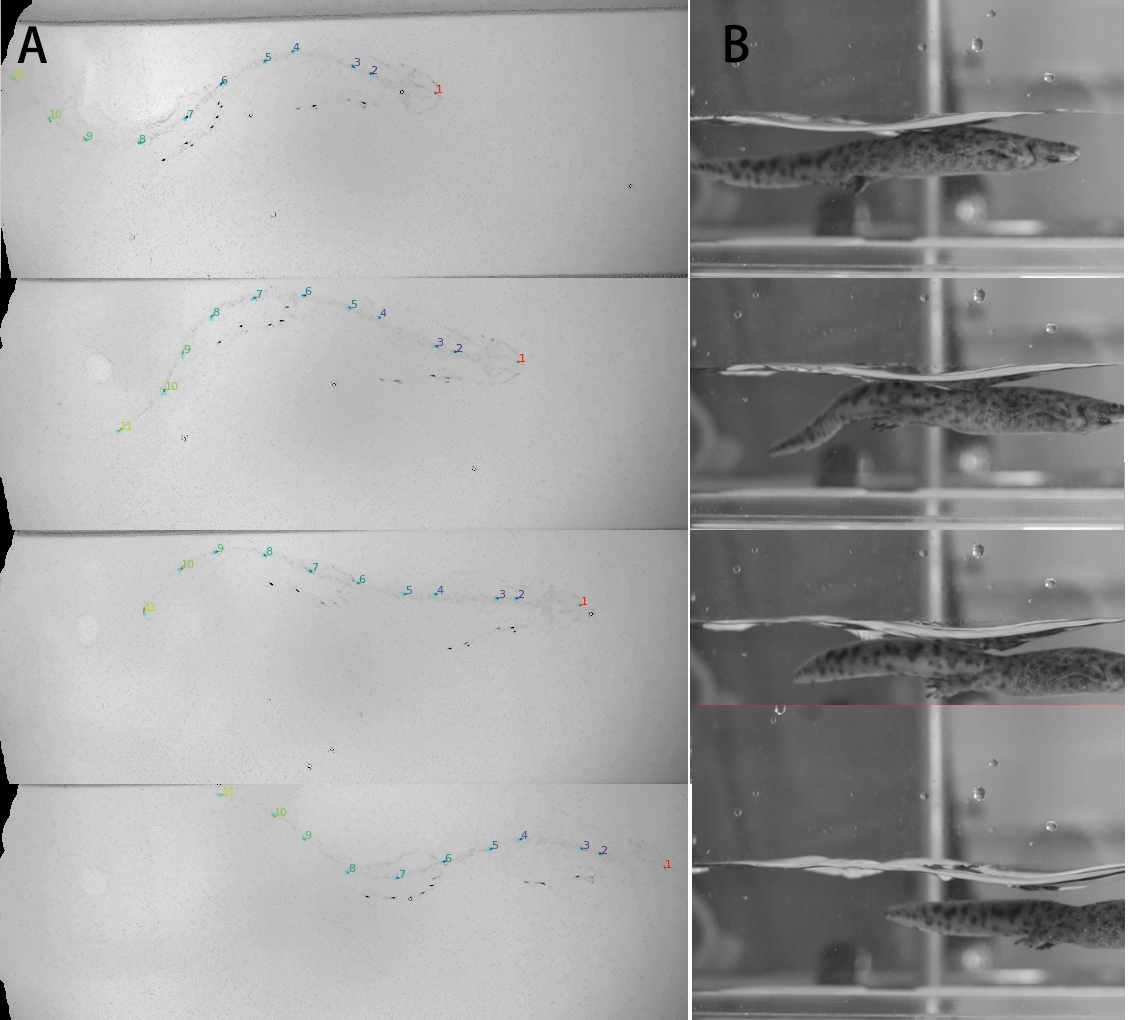
\includegraphics[width=.5\textwidth]{figures/imitation.png}
  \caption{\label{fig:imitation} A. Recorded swimming sequences of an adult female \textit{Salamander Pleurodeles Waltl} under X-ray B. Synchronized optical recording of swimming experiment.}
\end{figure}

Note that the robot is scaled up by a factor of 6.5 compared to the animal subject. To match their physical interactions with the environments, we need to apply a dynamical scaling \cite{karakasiliotis2016cineradiography}. For example, an equivalent robot frequency can be scaled as:

\begin{equation}
  \label{eq:dynamical scaling}
  f_{robot} = \sqrt{\frac{l_{salamander}}{l_{robot}}} \cdot f_{salamander}\\
\end{equation}



\textbf{\underline{Question 2.3} Analyze the provided animal data and compare the animal locomotion performance with your implemented controller in \fileref{\nolinkurl{cmc_controllers/exercise2.3.py}}. Back up your analysis with metrics.}

\underline{BONUS: Tune the controller to imitate the animal swimming behavior. Plot the animal kinematics} \\
\underline{and robot kinematics with quantified errors. (The bonus question would add to the project point if)} \\
\underline{properly solved. But the point cannot exceed the maximum possible point for Project 1)}



\subsection{Sensory feedback}
In this part, you will add stretch feedback to the open-loop CPG implemented in the previous section.

Stretch feedback is a form of local proprioceptive feedback from stretch-sensitive edge cells distributed along the spinal cord of the animal. Such sensory cells have been identified and described in the locomotor circuits of lamprey \cite{grillner1984edge} and zebrafish \cite{picton_spinal_2021}. In the case of the robot (Polymander) used in this project, stretch feedback is obtained from encoders mounted on each actuated servo motor. We simplify the model by considering only ipsilateral excitatory projections (i.e., stretch feedback activates neurons on the same side of the spinal cord).

We consider only stretch and ignore compression in this project.

\begin{equation}
  \label{eq:vartheta1}
  \vartheta_i(\text{left}) =
  \begin{cases}
    \theta_i, & \text{if } \theta_i > 0 \text{ (stretch)} \\
    0, & \text{otherwise}
  \end{cases}
\end{equation}

\begin{equation}
  \label{eq:vartheta2}
  \vartheta_i(\text{right}) =
  \begin{cases}
    -\theta_i, & \text{if } -\theta_i > 0 \text{ (stretch)} \\
    0, & \text{otherwise}
  \end{cases}
\end{equation}

which can be simplified as:
\begin{equation}
 \vartheta_i(\text{left}) = \max(0, \theta_i)
\end{equation}
\begin{equation}
  \vartheta_i(\text{right}) = \max(0, -\theta_i)
\end{equation}

The stretch feedback $s_i$ for oscillator $i$ is computed as the product of the stretch value $\vartheta_i$ and the feedback strength $w^{\text{ipsi}}$. To reduce the number of parameters, we use the same feedback strength for all segments:
\begin{equation}
  s_i = w^{\text{ipsi}} \vartheta_i
\end{equation}

After including stretch feedback, the oscillator equations are updated as:
\begin{equation}
  \dot{r}_i = a(R_i - r_i) + s_i \cos(\theta_i)
\end{equation}
where $r_i$ is the oscillator amplitude, $R_i$ the nominal amplitude, and $\theta_i$ the oscillator phase.

\begin{equation}
\label{eq:dtheta_sf}
  \dot{\theta}_i = 2 \pi f_i + \sum_j r_j w_{ij} \sin(\theta_j - \theta_i - \phi_{ij}) - \frac{s_i}{r_i} \sin(\theta_i)
\end{equation}
where $f_i$ is the oscillator frequency, $w_{ij}$ the coupling weights, and $\phi_{ij}$ the phase bias.

\textbf{\underline{Question 3.1}} Update \fileref{cmc\_controllers/CPG\_controller.py} to include stretch feedback. Run one simulation with feedback $w^{\text{ipsi}} = 3.0$ and another with $w^{\text{ipsi}} = 0$ using \fileref{scripts/exercise\_3.1.py}, and explain why it is interesting to vary these values.

Plot the time evolution of oscillator states ($\theta$ and $r$), the sum and difference of muscle outputs ($M_{L_i} + M_{R_i}$ and $M_{L_i} - M_{R_i}$), body joint angles, and the robot CoM trajectory in 2D. Compute the neural frequencies, neural amplitudes, forward speed, and CoT. Analyze how adding stretch feedback changes the simulation performance compared to the open-loop CPGs in \underline{Question 2.1}.

\textbf{Important:} Implement stretch feedback as an optional CPG parameter. Ensure that the implementation of the CPG from previous exercises (without stretch feedback) remains functional.

\textbf{Hint:} To reduce errors in neural metric computation, skip the transient phase (i.e., initial signals before reaching steady state). Increase the number of simulation steps and set the buffer size to $20001$ for better FFT resolution.


\textbf{\underline{Question 3.2}} Test different values of the ipsilateral feedback weight $w^{\text{ipsi}}$ in the range $[-3.0, 17.0]$ using \fileref{scripts/exercise\_3.2.py}. How does stretch feedback affect CoT, forward speed, neural frequency, and neural amplitude?

To model imperfections and noise in the neural network, we introduce neural disruptions to the robot controller as described in \cite{thandiackal2021emergence} (Fig.~3). Disruptions can be applied as \textbf{muted sensors}, \textbf{removed couplings}, or a combination of both.

The disruption is applied in the following steps:
\begin{itemize}
    \item Implement a disruption mask: create an array with the same shape as the disrupted objects, with values sampled uniformly between 0 and 1.
    \item Create a boolean mask to select disrupted elements where the mask value is smaller than the disruption probability $p_{\text{dist\_muted\_sensor}}$ or $p_{\text{dist\_removed\_coupling}}$. For simplicity, keep the disruption targets fixed throughout the simulation.
    \item For muted sensors, set the sensor values to zero.
    \item For removed couplings, set the caudal and rostral coupling strengths to zero (keep the contralateral coupling).
\end{itemize}

To study the robustness and redundancy of ipsilateral coupling in the CPG network, we carry out an ablation study with two controller configurations (Tab.~\ref{tab:disruption}) and five disruption probabilities equally distributed between $0\%$ and $15\%$ (Tab.~\ref{tab:disruption_config}).

\begin{table}[!ht]
\centering
\begin{tabular}{|l|l|l|}
    \hline
    Name & $disruption\_p\_sensors$ & $disruption\_p\_couplings$ \\
    \hline
    Muted Sensors & $[0,15\%]$ & $0$ \\
    \hline
    Removed Couplings & $0$ & $[0,15\%]$ \\
    \hline
    Mixed & \multicolumn{2}{c|}{$[0,15\%]$} \\
    \hline
\end{tabular}
\caption{\label{tab:disruption_config} Different disruption configurations}
\end{table}

\begin{table}[!ht]
\centering
\begin{tabular}{|l|l|l|}
    \hline
    Name & Sensory Feedback & Ipsilateral Coupling \\
    \hline
    Combined & + & + \\
    \hline
    Decoupled & + & - \\
    \hline
\end{tabular}
\caption{\label{tab:disruption} Different setups for the CPG controllers}
\end{table}




\textbf{\underline{Question 3.3}} Implement the neural disruptions in \fileref{scripts/exercise\_3.3.py}. Set the amplitude offset $c_{R_i,0}$ to $0$ and the feedback strength $w_{ipsi}$ to $10.0$. Run a longer simulation with $10{,}001$ steps (40\,s).
Explore the effect of disruption by simulating mixed disruption
configurations where \nolinkurl{disruption_p_sensors} and
\nolinkurl{disruption_p_couplings} are both set to $20\%$. What do you
observe in the simulation? How do the robot joint angles and trajectory
compare to the case without disruption?

For both the combined and decoupled network setups in Tab.~\ref{tab:disruption}, run simulations with five disruption probabilities as defined in Tab.~\ref{tab:disruption_config}. Plot the robot speed and CoT evolution.

\textbf{Hint:} For reproducible experiments, pass \texttt{random\_seed} to your controller initialization. Repeat the simulations with different seeds to obtain more general conclusions.




\bibliographystyle{ieeetr}
\bibliography{cmc_2026}
\label{sec:references}


\end{document}